\documentclass[tikz, convert={outfile=\jobname.png}]{standalone}

\usepackage{pgfplots}
\usepackage{tikz}
\usepackage{trfsigns}

\begin{document}


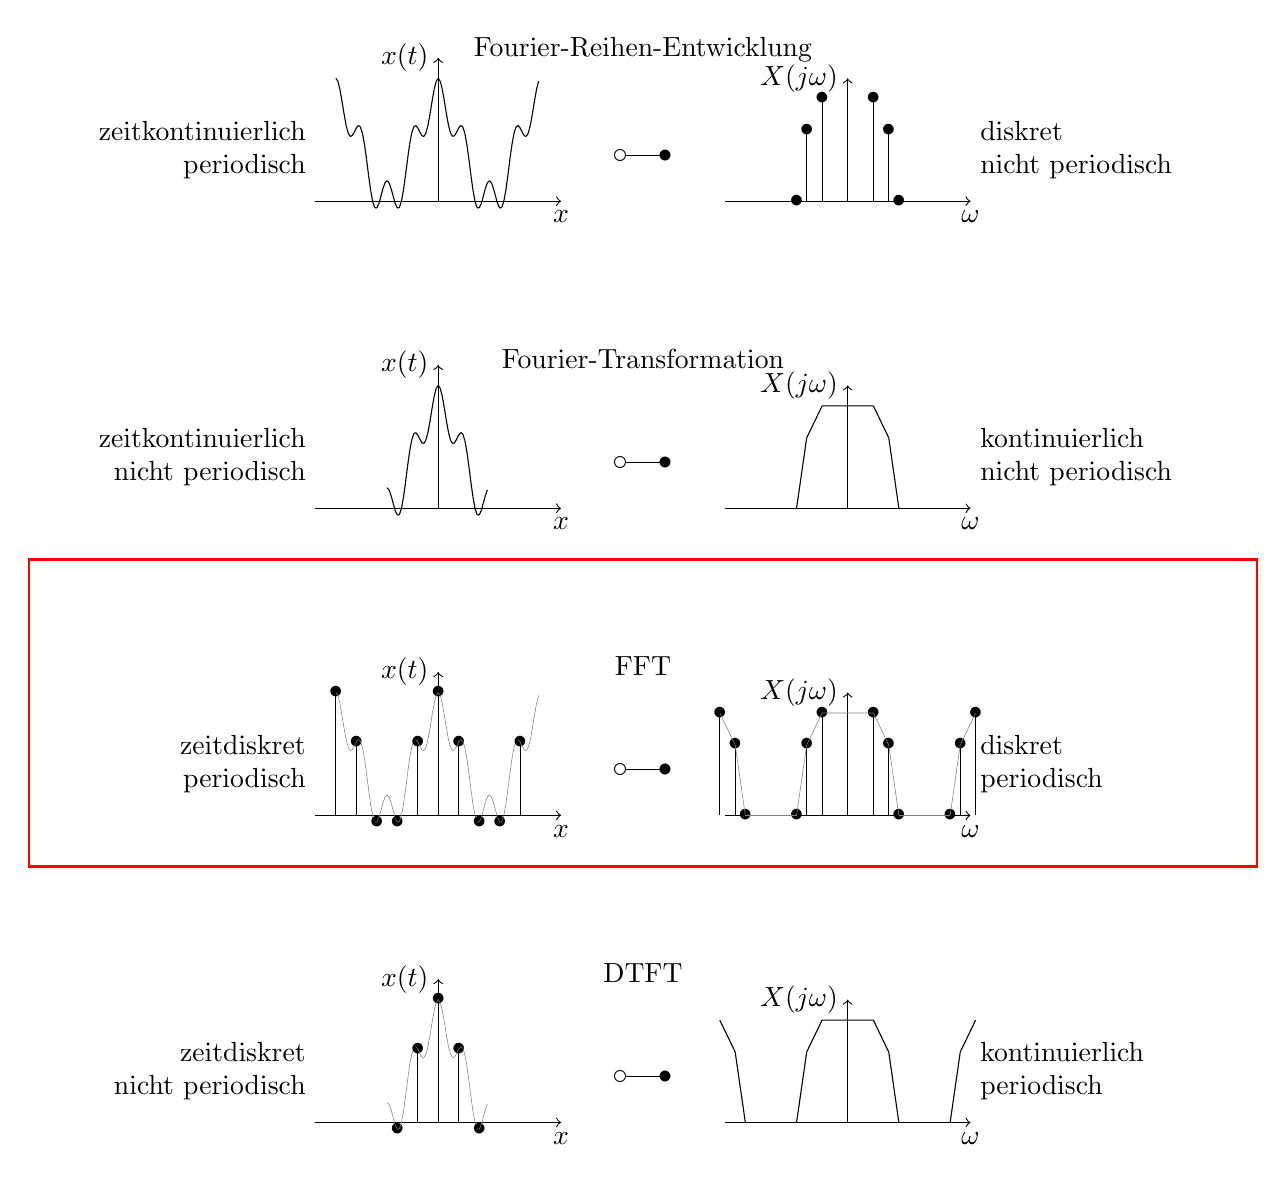
\begin{tikzpicture}[scale=1.3]
% periodisch % kontiniuierlich
\begin{scope}
\draw[->] (-1.2,0)--(1.2,0)node[below]{$x$};
\draw[->] (0,0)--(0,1.4)node[left]{$x(t)$};
\foreach\x[count = \i] in {-1,-.98,...,1}{
\pgfmathsetmacro{\y}{.5+.5*cos(180*2*\x)+.2*cos(180*2*\x*4)}
\ifnum\i > 1
\draw (last)--(\x,\y) node{};
\fi
\path(\x,\y) coordinate(last);
}
\path(-1.2,.5) node[align=right,left]{zeitkontinuierlich \\ periodisch};

% Spec
\path (2,0.5)node{$\laplace$}node[above=1cm]{Fourier-Reihen-Entwicklung};
\draw[->] (4-1.2,0)--(5.2,0)node[below]{$\omega$};
\draw[->] (4,0)--(4,1.2)node[left]{$X(j\omega)$};
\foreach\x[count = \i] in {3.5,3.6,3.75,4.25,4.4,4.5}{
\pgfmathsetmacro{\y}{1*sin(180*2*\x)^2+sin(180*2*\x*4)^2}
\draw[] (\x,0)--(\x,\y) node{$\bullet$};
}
\path(5.2,.5) node[align=left,right]{diskret \\ nicht periodisch};
\end{scope}


% periodisch % kontiniuierlich
\begin{scope}[xshift = 0cm, yshift = -3cm]
\draw[->] (-1.2,0)--(1.2,0)node[below]{$x$};
\draw[->] (0,0)--(0,1.4)node[left]{$x(t)$};
\foreach\x[count = \i] in {-.5,-.48,...,.5}{
\pgfmathsetmacro{\y}{.5+.5*cos(180*2*\x)+.2*cos(180*2*\x*4)}
\ifnum\i > 1
\draw (last)--(\x,\y) node{};
\fi
\path(\x,\y) coordinate(last);
}
\path(-1.2,.5) node[align=right,left]{zeitkontinuierlich \\ nicht periodisch};

% Spec
\path (2,0.5)node{$\laplace$}node[above=1cm]{Fourier-Transformation};
\draw[->] (4-1.2,0)--(5.2,0)node[below]{$\omega$};
\draw[->] (4,0)--(4,1.2)node[left]{$X(j\omega)$};
\foreach\x[count = \i] in {3.5,3.6,3.75,4.25,4.4,4.5}{
\pgfmathsetmacro{\y}{1*sin(180*2*\x)^2+sin(180*2*\x*4)^2}
%\draw[help lines] (\x,0)--(\x,\y) node{$\bullet$};
\ifnum\i > 1
\draw (last)--(\x,\y) node{};
\fi
\path(\x,\y) coordinate(last);
}
\path(5.2,.5) node[align=left,right]{kontinuierlich \\ nicht periodisch};
\end{scope}



% FFT
\begin{scope}[yshift = -6cm]
\draw[->] (-1.2,0)--(1.2,0)node[below]{$x$};
\draw[->] (0,0)--(0,1.4)node[left]{$x(t)$};
\foreach\x[count = \i] in {-1,-.98,...,1}{
\pgfmathsetmacro{\y}{.5+.5*cos(180*2*\x)+.2*cos(180*2*\x*4)}
\pgfmathtruncatemacro{\dec}{mod((\i-1),10)}
\ifnum\dec = 0
\draw[] (\x,0)--(\x,\y)node{$\bullet$};
\fi
\ifnum\i > 1
\draw[help lines] (last)--(\x,\y) node{};
\fi
\path(\x,\y) coordinate(last);
}
\path(-1.2,.5) node[align=right,left]{zeitdiskret \\ periodisch};

% Spec
\path (2,0.5)node{$\laplace$}node[above=1cm]{FFT};
\draw[->] (4-1.2,0)--(5.2,0)node[below]{$\omega$};
\draw[->] (4,0)--(4,1.2)node[left]{$X(j\omega)$};
\foreach\x[count = \i] in {2.75,2.9,3,3.5,3.6,3.75,4.25,4.4,4.5,5,5.1,5.25}{
\pgfmathsetmacro{\y}{1*sin(180*2*\x)^2+sin(180*2*\x*4)^2}
\draw[] (\x,0)--(\x,\y) node{$\bullet$};
\ifnum\i > 1
\draw[help lines] (last)--(\x,\y) node{};
\fi
\path(\x,\y) coordinate(last);
}
\path(5.2,.5) node[align=left,right]{diskret \\ periodisch};

\draw[thick,red](-4,-.5)rectangle(8,2.5);
\end{scope}


% DTFT
\begin{scope}[yshift = -9cm]
\draw[->] (-1.2,0)--(1.2,0)node[below]{$x$};
\draw[->] (0,0)--(0,1.4)node[left]{$x(t)$};
\foreach\x[count = \i] in {-.5,-.48,...,.5}{
\pgfmathsetmacro{\y}{.5+.5*cos(180*2*\x)+.2*cos(180*2*\x*4)}
\pgfmathtruncatemacro{\dec}{mod((\i-6),10)}
\ifnum\dec = 0
\draw[] (\x,0)--(\x,\y)node{$\bullet$};
\fi
\ifnum\i > 1
\draw[help lines] (last)--(\x,\y) node{};
\fi
\path(\x,\y) coordinate(last);
}
\path(-1.2,.5) node[align=right,left]{zeitdiskret \\ nicht periodisch};

% Spec
\path (2,0.5)node{$\laplace$}node[above=1cm]{DTFT};
\draw[->] (4-1.2,0)--(5.2,0)node[below]{$\omega$};
\draw[->] (4,0)--(4,1.2)node[left]{$X(j\omega)$};
\foreach\x[count = \i] in {2.75,2.9,3,3.5,3.6,3.75,4.25,4.4,4.5,5,5.1,5.25}{
\pgfmathsetmacro{\y}{1*sin(180*2*\x)^2+sin(180*2*\x*4)^2}
\ifnum\i > 1
\draw[] (last)--(\x,\y) node{};
\fi
\path(\x,\y) coordinate(last);
}
\path(5.2,.5) node[align=left,right]{kontinuierlich \\ periodisch};
\end{scope}
\end{tikzpicture}
%

\end{document}